\chapterimage{operator.jpg} % Chapter heading image

\chapter{Ponteiros e Arrays}
Ok, vamos em frente. Vamos considerar porque precisamos identificar o tipo de variável para a qual um ponteiro aponta, como em:
\begin{lstlisting}
	int *ptr;
\end{lstlisting}

Uma razão para fazer isso é que mais tarde, uma vez que \textbf{ptr} ``aponta para'' algo, se escrevermos:
\begin{lstlisting}
	*ptr = 2;
\end{lstlisting}
o compilador saberá quantos bytes copiar para aquele local de memória apontado por \textbf{ptr}. Se \textbf{ptr} for declarado apontando para um inteiro, 4 bytes serão copiados, se for longo, 8 bytes serão copiados. Da mesma forma, para \textit{floats} e \textit{doubles}, o número apropriado será copiado. Porém, definir o tipo para o qual o ponteiro aponta permite uma série de outras maneiras interessantes que um compilador pode interpretar o código. Por exemplo, considere um bloco na memória consistindo em dez inteiros em uma linha. Ou seja, 40 bytes de memória são reservados para conter 10 inteiros.

Agora, digamos que apontamos nosso ponteiro de inteiro \textbf{ptr} para o primeiro desses inteiros. Além disso, digamos que o inteiro esteja localizado na posição de memória 100 (decimal). O que acontece quando escrevemos:
\begin{lstlisting}
	ptr + 1;
\end{lstlisting}

Porque o compilador ``sabe'' que este é um ponteiro (ou seja, seu valor é um endereço) e que aponta para um inteiro (seu endereço atual, 100, é o endereço de um inteiro), ele adiciona 4 a \textbf{ptr} em vez de 1, então o ponteiro ``aponta para'' o \textbf{próximo inteiro}, no local da memória 104. Da mesma forma, se o \textbf{ptr} fosse declarado como um ponteiro para um longo, ele adicionaria 8 a ele em vez de 1.
O mesmo vale para outros tipos de dados, como floats, doubles ou até mesmo tipos de dados definidos pelo usuário, como estruturas. Obviamente, esse não é o mesmo tipo de ``adição'' em que normalmente pensamos. Em C, é referido como adição usando ``aritmética de ponteiros'', um termo ao qual voltaremos mais tarde.

Da mesma forma, uma vez que \textbf{++ptr} e \textbf{ptr++} são ambos equivalentes a \textbf{ptr + 1} (embora o ponto no programa quando \textbf{ptr} é incrementado possa ser diferente), incrementar um ponteiro usando o operador unário \textbf{++}, seja pré- ou pós-, incrementa o endereço que ele armazena pela quantidade \textit{sizeof(tipo)} onde ``tipo'' é o tipo do objeto apontado. (ou seja, 4 para um número inteiro, 8 para um longo, etc.).

Como um bloco de 10 inteiros localizado contiguamente na memória é, por definição, um array de inteiros, isso traz uma relação interessante entre arrays e ponteiros.

Considere o seguinte:
\begin{lstlisting}
	int meu_array[] = {1,23,17,4,-5,100};
\end{lstlisting}

Aqui temos um array contendo 6 inteiros. Referimo-nos a cada um desses inteiros por meio de um subscrito para \textbf{meu\_array}, ou seja, usando de \textbf{meu\_array[0]} até \textbf{meu\_array[5]}. Mas, podemos acessá-los alternativamente por meio de um ponteiro da seguinte maneira:

\begin{lstlisting}
	int *ptr;
	ptr = &meu_array[0]; /* o ponteiro aponta para o primeiro
	                        inteiro em nosso array */
\end{lstlisting}

E então poderíamos imprimir nosso array usando a notação de array ou desreferenciando nosso ponteiro. O código a seguir ilustra isso:

\lstinputlisting[caption=Ponteiros e arrays, numbers=left]{code/prog2-1.c}

Compile e execute o programa acima e observe cuidadosamente as linhas A e B e que o programa imprime os mesmos valores em ambos os casos. Observe também como desreferenciamos nosso ponteiro na linha B, ou seja, primeiro adicionamos \textbf{i} a ele e, em seguida, desreferenciamos o novo ponteiro.
Se você digitou o programa corretamente, sua sáida deve ser algo como:
\lstconsolestyle
\begin{lstlisting}
meu_array[0] = 1	ptr + 0 = 1
meu_array[1] = 23	ptr + 1 = 23
meu_array[2] = 17	ptr + 2 = 17
meu_array[3] = 4	ptr + 3 = 4
meu_array[4] = -5	ptr + 4 = -5
meu_array[5] = 100	ptr + 5 = 100
\end{lstlisting}
\lstcodestyle

Mude a linha B para:
\begin{lstlisting}
	printf("ptr + %d = %d\n",i, *ptr++);
\end{lstlisting}
e execute-o novamente ... depois mude para:
\begin{lstlisting}
	printf("ptr + %d = %d\n",i, *(++ptr));
\end{lstlisting}
e tente mais uma vez. A cada vez, tente prever o resultado e observe cuidadosamente o resultado real.

Em C, o padrão afirma que onde quer que possamos usar \textbf{\&var\_nome[0]}, podemos substituir isso por \textbf{var\_nome}, portanto, em nosso código onde escrevemos:
\begin{lstlisting}
	ptr = &meu_array[0];
\end{lstlisting}
podemos escrever:
\begin{lstlisting}
	ptr = meu_array;
\end{lstlisting}
para alcançar o mesmo resultado.

Isso leva muitos textos a afirmar que o nome de um array é um ponteiro. Eu prefiro pensar mentalmente ``o nome do array é o endereço do primeiro elemento no array". Muitos iniciantes (incluindo eu quando estava aprendendo) tendem a ficar confusos pensando nisso como um ponteiro. Por exemplo, enquanto podemos escrever
\begin{lstlisting}
	ptr = meu_array;
\end{lstlisting}
mas não podemos escrever
\begin{lstlisting}
	meu_array = ptr;
\end{lstlisting}

O motivo é que, embora \textbf{ptr} seja uma variável, \textbf{meu\_array} é uma constante. Ou seja, o local em que o primeiro elemento de \textbf{meu\_array} será armazenado não pode ser alterado depois que \textbf{meu\_array[]} for declarado.

A Figura \ref{fig:pontarrays} mostra uma possível configuração dessas variáveis.
\begin{figure}[ht]
	\begin{center}
		% Graphic for TeX using PGF
% Title: /home/araujo/Dropbox/VerbTeX/LivroComputadores/Pictures/memoria.dia
% Creator: Dia v0.97.3
% CreationDate: Sun May 21 11:59:17 2017
% For: araujo
% \usepackage{tikz}
% The following commands are not supported in PSTricks at present
% We define them conditionally, so when they are implemented,
% this pgf file will use them.
\ifx\du\undefined
  \newlength{\du}
\fi
\setlength{\du}{15\unitlength}
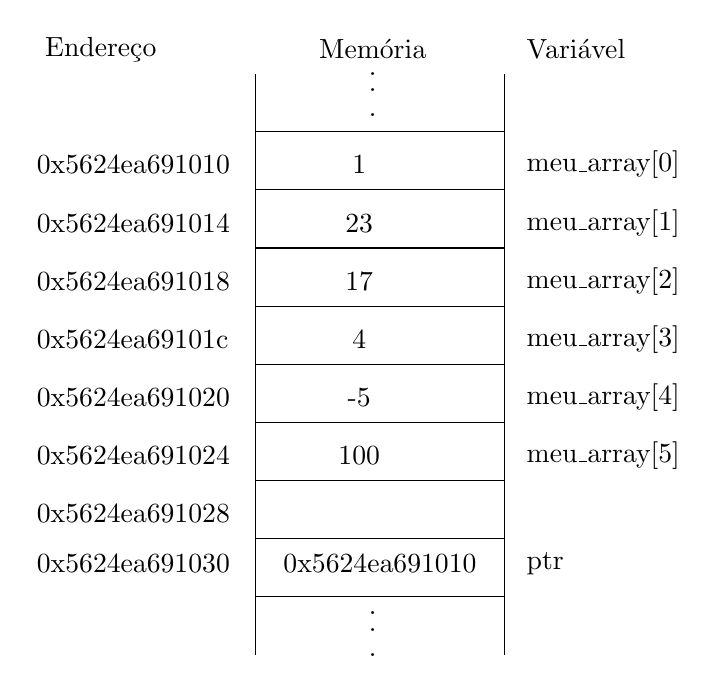
\begin{tikzpicture}
\pgftransformxscale{1.000000}
\pgftransformyscale{-1.000000}
\definecolor{dialinecolor}{rgb}{0.000000, 0.000000, 0.000000}
\pgfsetstrokecolor{dialinecolor}
\definecolor{dialinecolor}{rgb}{1.000000, 1.000000, 1.000000}
\pgfsetfillcolor{dialinecolor}

\draw (31\du,9.4\du)--(31.\du,8\du)--(25\du,8\du)--(25\du,9.4\du);
\node at (27.5\du,8.8\du){1};
\draw (31\du,10.8\du)--(31.\du,9.4\du)--(25\du,9.4\du)--(25\du,10.8\du);
\node at (27.5\du,10.2\du){23};
\draw (31\du,12.2\du)--(31.\du,10.8\du)--(25\du,10.8\du)--(25\du,12.2\du);
\node at (27.5\du,11.6\du){17};
\draw (31\du,13.6\du)--(31.\du,12.2\du)--(25\du,12.2\du)--(25\du,13.6\du);
\node at (27.5\du,13\du){4};
\draw (31\du,15\du)--(31.\du,13.6\du)--(25\du,13.6\du)--(25\du,15\du);
\node at (27.5\du,14.4\du){-5};
\draw (31\du,16.4\du)--(31.\du,15\du)--(25\du,15\du)--(25\du,16.4\du);
\node at (27.5\du,15.8\du){100};
\draw (31\du,17.8\du)--(31.\du,16.4\du)--(25\du,16.4\du)--(25\du,17.8\du);
\node at (28\du,18.4\du){0x5624ea691010};
\draw (31\du,17.8\du)--(31.\du,16.4\du)--(25\du,16.4\du)--(25\du,17.8\du);
%\node at (27.5\du,18.6\du){0110 1100};
\draw (31\du,19.2\du)--(31.\du,17.8\du)--(25\du,17.8\du)--(25\du,19.2\du)--cycle;
\node[anchor=west] at (27.5\du,20.6\du){.};
\node[anchor=west] at (27.5\du,20\du){.};
\node[anchor=west] at (27.5\du,19.6\du){.};

\definecolor{dialinecolor}{rgb}{0.000000, 0.000000, 0.000000}
\pgfsetstrokecolor{dialinecolor}
\draw (25\du,19.2\du)--(25\du,20.6\du);
\draw (31\du,19.2\du)--(31\du,20.6\du);
\draw (25\du,6.6\du)--(25\du,8\du);
\draw (31\du,6.6\du)--(31\du,8\du);
\node[anchor=west] at (27.5\du,7.600000\du){.};
\node[anchor=west] at (27.5\du,7.000000\du){.};
\node[anchor=west] at (27.5\du,6.600000\du){.};
\node[anchor=west] at (19.5\du,8.8\du){0x5624ea691010};
\node[anchor=west] at (19.5\du,10.2\du){0x5624ea691014};
\node[anchor=west] at (19.5\du,11.6\du){0x5624ea691018};
\node[anchor=west] at (19.5\du,13\du){0x5624ea69101c};
\node[anchor=west] at (19.5\du,14.4\du){0x5624ea691020};
\node[anchor=west] at (19.5\du,15.8\du){0x5624ea691024};
\node[anchor=west] at (19.5\du,17.2\du){0x5624ea691028};
\node[anchor=west] at (19.5\du,18.4\du){0x5624ea691030};
\node[anchor=west] at (19.7\du,6.002347\du) {Endere\c{c}o};
\node[anchor=west] at (26.3\du,6.002347\du){Mem\'{o}ria};
\node[anchor=west] at (31.3\du,6.002347\du){Vari\'{a}vel};
\node[anchor=west] at (31.3\du,8.8\du){meu\_array[0]};
\node[anchor=west] at (31.3\du,10.2\du){meu\_array[1]};
\node[anchor=west] at (31.3\du,11.6\du){meu\_array[2]};
\node[anchor=west] at (31.3\du,13\du){meu\_array[3]};
\node[anchor=west] at (31.3\du,14.4\du){meu\_array[4]};
\node[anchor=west] at (31.3\du,15.8\du){meu\_array[5]};
\node[anchor=west] at (31.3\du,18.4\du){ptr};
\end{tikzpicture}

		\caption{Ponteiros e arrays.}
		\label{fig:pontarrays}
	\end{center}
\end{figure}

Anteriormente, ao discutir o termo ``lvalue'', citei K\&R-2, onde afirmava:

\begin{quotation}
	``Um \textbf{objeto} é uma região nomeada de armazenamento; um \textbf{lvalue} é uma expressão que se refere a um objeto''.
\end{quotation}

Isso levanta um problema interessante. Visto que \textbf{meu\_array} é uma região nomeada de armazenamento, por que \textbf{meu\_array} na instrução de atribuição acima não é um \textit{lvalue}? Para resolver esse problema, alguns se referem a \textbf{meu\_array} como um ``\textit{lvalue} não modificável''.

Modifique o programa de exemplo anterior mudando
\begin{lstlisting}
	ptr = &meu_array[0];
\end{lstlisting}
para
\begin{lstlisting}
	ptr = meu_array;
\end{lstlisting}
e execute-o novamente para verificar se os resultados são idênticos.

Agora, vamos nos aprofundar um pouco mais na diferença entre os nomes \textbf{ptr} e \textbf{meu\_array} como usados acima. Alguns escritores se referem ao nome de um array como um ponteiro constante. O que queremos dizer com isso? Bem, para entender o termo ``\textbf{\textit{constante}}'' neste sentido, vamos voltar à nossa definição do termo ``variável''. Quando declaramos uma variável, reservamos um ponto na memória para armazenar o valor do tipo apropriado. Feito isso, o nome da variável pode ser interpretado de duas maneiras. Quando usado no lado esquerdo do operador de atribuição, o compilador o interpreta como o local da memória para o qual mover aquele valor resultante da avaliação do lado direito do operador de atribuição. Mas, quando usado no lado direito do operador de atribuição, o nome de uma variável é interpretado como significando o conteúdo armazenado naquele endereço de memória reservado para conter o valor dessa variável.

Com isso em mente, vamos agora considerar a mais simples das constantes, como em:
\begin{lstlisting}
	int i, k;
	i = 2;
\end{lstlisting}

Aqui, enquanto \textbf{i} é uma variável e então ocupa espaço na porção de dados da memória, 2 é uma constante e, como tal, em vez de reservar memória no segmento de dados, é embutido diretamente no segmento de código da memória. Ou seja, ao escrever algo como \textbf{k = i;} dizemos ao compilador para criar um código que, em tempo de execução, examinará a localização da memória \textbf{\&i} para determinar o valor a ser movido para \textbf{k}, o código criado por \textbf{i = 2;} simplesmente coloca o 2 no código e não há referência ao segmento de dados. Ou seja, \textbf{k} e \textbf{i} são objetos, mas 2 não é um objeto.

Da mesma forma, no exemplo acima, uma vez que \textbf{meu\_array} é uma constante, uma vez que o compilador estabelece onde o próprio \textit{array} deve ser armazenado, ele ``sabe'' o endereço de \textbf{meu\_array[0]} e ao ver:
\begin{lstlisting}
	ptr = meu_array;
\end{lstlisting}
ele simplesmente usa esse endereço como uma constante no segmento de código e não há referência do segmento de dados além disso.

Este pode ser um bom lugar para explicar melhor o uso da expressão \textbf{(void *)} usada no Programa \ref{prog1-1} do Capítulo 1. Como vimos, podemos ter ponteiros de vários tipos. Até agora, discutimos ponteiros para inteiros e ponteiros para caracteres. Nos próximos capítulos, aprenderemos sobre ponteiros para estruturas e até mesmo ponteiros para ponteiros.

Também aprendemos que em diferentes sistemas o tamanho de um ponteiro pode variar. Acontece que também é possível que o tamanho de um ponteiro possa variar dependendo do tipo de dados do objeto para o qual ele aponta. Assim, como acontece com inteiros nos quais você pode ter problemas ao tentar atribuir um inteiro longo a uma variável do tipo inteiro curto, você pode ter problemas ao tentar atribuir os valores de ponteiros de vários tipos a variáveis de ponteiro de outros tipos.

Para minimizar esse problema, C fornece um ponteiro do tipo \textbf{void}. Podemos declarar tal ponteiro escrevendo:
\begin{lstlisting}
	void *vptr;
\end{lstlisting}

Um ponteiro \textbf{void} é uma espécie de ponteiro genérico. Por exemplo, enquanto C não permite a comparação de um ponteiro para um tipo inteiro com um ponteiro para um tipo caractere, por exemplo, qualquer um deles pode ser comparado a um ponteiro \textbf{void}. Claro, como com outras variáveis, os \textit{casts} podem ser usados para converter de um tipo de ponteiro para outro nas circunstâncias adequadas. No Programa \ref{prog1-1} do Capítulo 1, converto os ponteiros para inteiros em ponteiros vazios para torná-los compatíveis com a especificação de conversão \textbf{\%p}. Em capítulos posteriores, outros \textit{casts} serão feitos pelas razões aqui definidas.

Bem, isso é muito material técnico para digerir e não espero que um iniciante entenda tudo isso na primeira leitura. Com o tempo e experimentação, você vai querer voltar e reler os primeiros 2 capítulos. Mas, por enquanto, vamos prosseguir para a relação entre ponteiros, arrays de caracteres e strings.

